
\begin{center}
\textit{\textbf{Corrigé officiel (éduscol)}}
\end{center}

\textbf{Question 1}

\medskip

\begin{enumerate}
\item L'équation réduite de la tangente à une courbe de la fonction $f$ au point A$(1~;~0)$ est :
\[y = f'(1)(x - 1) + 0.\]
Or $f'(x) = \dfrac{1}{x}$ donc $f'(1) = 1$ et l'équation réduite cherchée est $y = x - 1$.
\item L'aire de $A_1$ est donnée par la formule $\dfrac{h(b+B)}{2}$ où
$h = 2\ln(3), \, b = 8 - 2\ln(3)$ et $B = 8$.

En remplaçant dans la formule et en réduisant on retrouve bien $16 \ln(3) - 2 (\ln(3))^2$.
\end{enumerate}

\bigskip

\textbf{Question 2}

\medskip

\begin{enumerate}
\item Lorsqu'on donne l'instruction \texttt{meth\_rect(2)}, le pas choisi est de 2 -- contrairement aux figures 3 et 5 -- et le premier rectangle est construit avec $x = 1$ et est donc aplati, contrairement à la figure 2. C'est donc la figure 4 qui représente la situation calculée par \texttt{meth\_rect(2)}.

\item D'après l'analyse faite à la question \textbf{1.}, la méthode des rectangles implémentée en Python donne une valeur inférieure à $A_2$ donc $A_2 > \texttt{9.307920700315046}$.
\end{enumerate}

\bigskip

\textbf{Question 3}

\medskip

\begin{enumerate}
\item On commence par dériver la fonction $x \mapsto x \ln(x)$ comme produit de deux fonctions puis on obtient, pour tout réel $x$ de l'intervalle $[1~;~9]$,
 
$F'(x) = \ln(x) = f(x)$ et $F$ est donc une primitive de $f$ sur $[1~;~9]$.

\item $A_2$ est l'aire du domaine délimité par l'axe des abscisses, la courbe de la fonction $f$ et la droite verticale d'équation $x = 9$.
 
De plus $f$ est positive sur $[1~;~9]$ et $f(1) = 0$.

Comme la fonction $f$ est dérivable sur $[1~;~9]$,

$A_2 = \int_{1}^{9} f(x) dx$.

Enfin, $F$ étant une primitive de $f$ sur l'intervalle $[1~;~9]$,  

$A_2 = F(9) - F(1)$ soit $A_2 = 9 \ln(9) - 10 = 18 \ln(3) - 10$.
\end{enumerate}

\bigskip

\textbf{Question 4}

\medskip

\begin{enumerate}
\item Pour tout réel $x$, $f'(x) = (3 - 3x - 2)\e^x = (-3x + 1)\e^x$.

\item La fonction exponentielle étant strictement positive sur $\mathbb{R}$, le signe de $f'(x)$ est celui de $-3x + 1$.
\begin{center}
\begin{tikzpicture}
\tkzTabInit[lgt=2.5, espcl=3]{$x$ / 1, {Signe de $-3x + 1$} / 1, {Variations de $f$} / 2}{${-\infty}$, ${\frac13}$, ${+\infty}$}
\tkzTabLine{,+,0,-,}
\tkzTabVar{-/{$$},+/{$$},-/{$$}}{/}
\end{tikzpicture}
\end{center}
\end{enumerate}

\bigskip

\textbf{Question 5}

\medskip

La formule d'Al-Kashi, appliquée au triangle PQR permet de calculer la longueur PR : 
\[\text{PR}^2 = \text{PQ}^2 + \text{QR}^2 - 2\text{PQ} \times \text{QR} \times \cos(\widehat{\text{PQR}})\]

Puis après application numérique : $\text{PR}^2 = 5^2 + 3^2 - 2 \times 5 \times 3 \times \cos\dfrac{\pi}{3}$

Pour finir, $\text{PR}^2 = 19$ soit $\text{PR} = \sqrt{19}$.

\bigskip

\textbf{Question 6}

\medskip

\begin{enumerate}
\item Pour tout réel $t$, $f'(t) = -3 \sin(3t + \varphi)$
et donc $f''(t) = -9 \cos(3t + \varphi)$.

Donc pour tout réel $t$, $f''(t) + 9f(t) = -9 \cos(3t + \varphi) + 9 \cos(3t + \varphi) = 0$.
\item $f(0) = \dfrac{\sqrt{2}}{2} \iff \cos\varphi = \dfrac{\sqrt{2}}{2} \iff \varphi = \dfrac{\pi}{4} \text{ car } \varphi \in [0~;~\pi[$.
\end{enumerate}

\bigskip


